\documentclass[12pt,a4paper]{article}
\usepackage{graphicx}
\setlength{\textwidth}{190mm}
\setlength{\textheight}{253mm}
\setlength{\oddsidemargin}{-14mm}
\setlength{\evensidemargin}{-14mm}
\setlength{\topmargin}{-12mm}

\setlength{\parindent}{0pt}
\setlength{\parskip}{1ex plus 0.5ex minus 0.2ex}

\setcounter{secnumdepth}{-1}   % disable section numbering

\newcommand{\E}{\mathrm{E}}
\newcommand{\C}{\mathrm{C}}
\newcommand{\dd}[2]{\frac{\partial{#1}}{\partial{#2}}}

\begin{document}
\title{Corrected error calculation for iterative Bayesian unfolding}
\author{Tim Adye, Rutherford Appleton Laboratory}
\date{4th February 2011}
\maketitle

The unfolding method based on iterative application of Bayes' theorem
described by D'Agostini~\cite{D'Agostini:1994zf}
(though similar to the iterative procedure of
M\"ulthei and Schorr~\cite{Multhei:1986ps})
is a convenient method, popular in Particle Physics.

\subsection{Measurement uncertainties}

As with all unfolding methods, it is important to understand
the uncertainties in the unfolded distribution, and especially the bin-to-bin correlations
that ensue as a result of the regularisation process (in the Bayes method without additional smoothing, regularisation
comes about as a result of limiting the number of iterations).
In many cases, the largest source of uncertainty is from propagation of the measurement
uncertainties through the unfolding matrix.

D'Agostini (\cite{D'Agostini:1994zf}~section~4) gives the unfolded distribution (``estimated causes''), $\hat{n}(\C_i)$,
as the result of applying the unfolding matrix, $M_{ij}$, to the measurements (``effects''), $n(\E_j)$:

\begin{equation}
\hat{n}(\C_i) = \sum_{j=1}^{n_{\E}} M_{ij} n(\E_j)
\label{eq:nCi}
\end{equation}

\noindent where

\begin{equation}
M_{ij} = \frac{P(\E_j|\C_i) P_0(\C_i)}{[\sum_{l=1}^{n_{\E}} P(\E_l|\C_i)] [\sum_{l=1}^{n_{\C}} P(\E_j|\C_l) P_0(C_l)]}
\end{equation}

\noindent and $P(\E_j|\C_i)$ is the response matrix, $\epsilon_i \equiv \sum_{j=1}^{n_{\E}} P(\E_j|\C_i)$ are the efficiencies,
and $P_0(C_l)$ is the prior distribution --- initially arbitrary (eg. flat or MC model), but updated on
subsequent iterations.

D'Agostini then calculates the covariance matrix, which here we call $V(\hat{n}(\C_k),\hat{n}(\C_l))$,
by error propagation from $n(\E_j)$,
but assumes that $M_{ij}$ is itself independent of $n(\E_j)$. That is only true for the first iteration.
For subsequent iterations, $P_0(\C_i)$ is replaced by $\hat{n}(\C_i) / \hat{N}_{\mathrm{true}}$
($\hat{N}_{\mathrm{true}} \equiv \sum_{i=1}^{n_{\C}} \hat{n}(\C_i)$) from the
previous iteration, and $\hat{n}(\C_i)$ depends on $n(\E_j)$ (eq.~\ref{eq:nCi}).

To take this into account, we compute the error propagation matrix

\begin{equation}
\dd{\hat{n}(\C_i)}{n(\E_j)} = M_{ij} + \sum_{k=1}^{n_{\E}} M_{ik} n(\E_k)
\left( \frac{1}{n_0(\C_i)} \dd{n_0(\C_i)}{n(\E_j)} - \sum_{l=1}^{n_{\C}} \frac{\epsilon_l}{n_0(\C_l)} \dd{n_0(\C_l)}{n(\E_j)} M_{lk} \right)
\label{eq:dnCidnEj}
\end{equation}

This depends upon the matrix $\dd{n_0(\C_i)}{n(\E_j)}$ which is $\dd{\hat{n}(\C_i)}{n(\E_j)}$ from the previous iteration.
In the first iteration, the second term vanishes ($\dd{n_0(\C_i)}{n(\E_j)}=0$) and we get $\dd{\hat{n}(\C_i)}{n(\E_j)} = M_{ij}$.

We can use the error propagation matrix to obtain the covariance matrix on the unfolded distribution

\begin{equation}
V(\hat{n}(\C_k),\hat{n}(\C_l)) = \sum_{i,j=1}^{n_{\E}} \dd{\hat{n}(\C_k)}{n(\E_i)} V(n(\E_i),n(\E_j)) \dd{\hat{n}(\C_l)}{n(\E_j)}
\label{eq:Vij}
\end{equation}

\noindent from the covariance matrix of the measurements, $V(n(\E_i),n(\E_j))$.

Without the new second term in eq.~\ref{eq:dnCidnEj},
the error is underestimated if more than one iteration
is used, but agrees well with toy Monte Carlo tests if the full error propagation is used
(see figure~\ref{fig:bayes_errors}).%
\begin{figure}[ht]
\makebox[\textwidth]{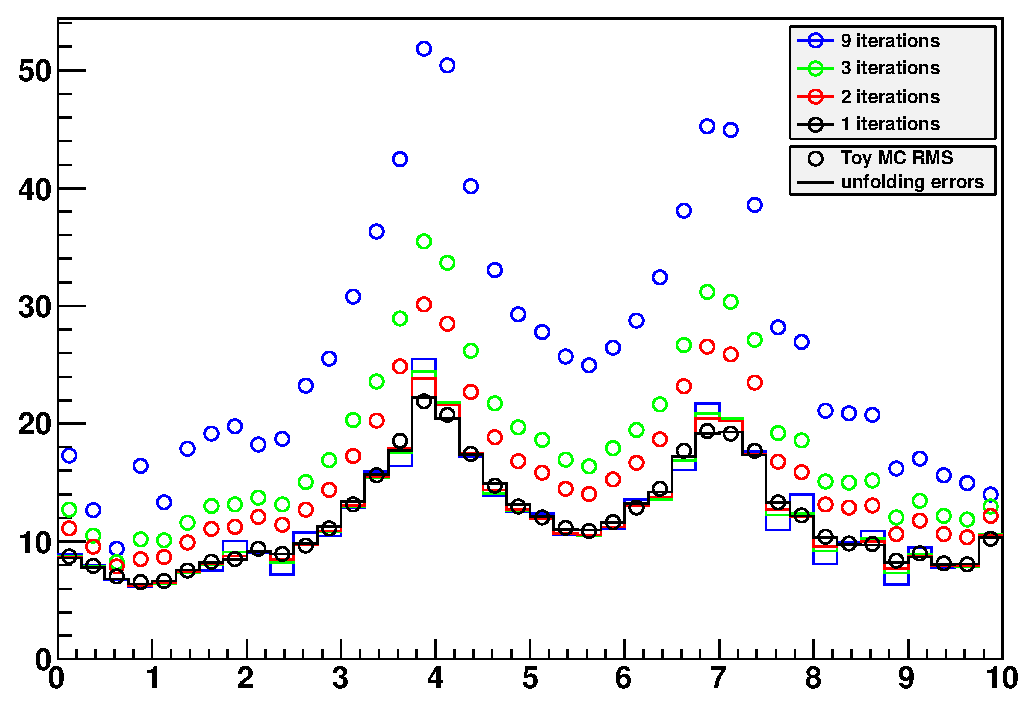
\includegraphics[width=.47\textwidth,clip]{bayes_errors_old.eps}\hfill
                     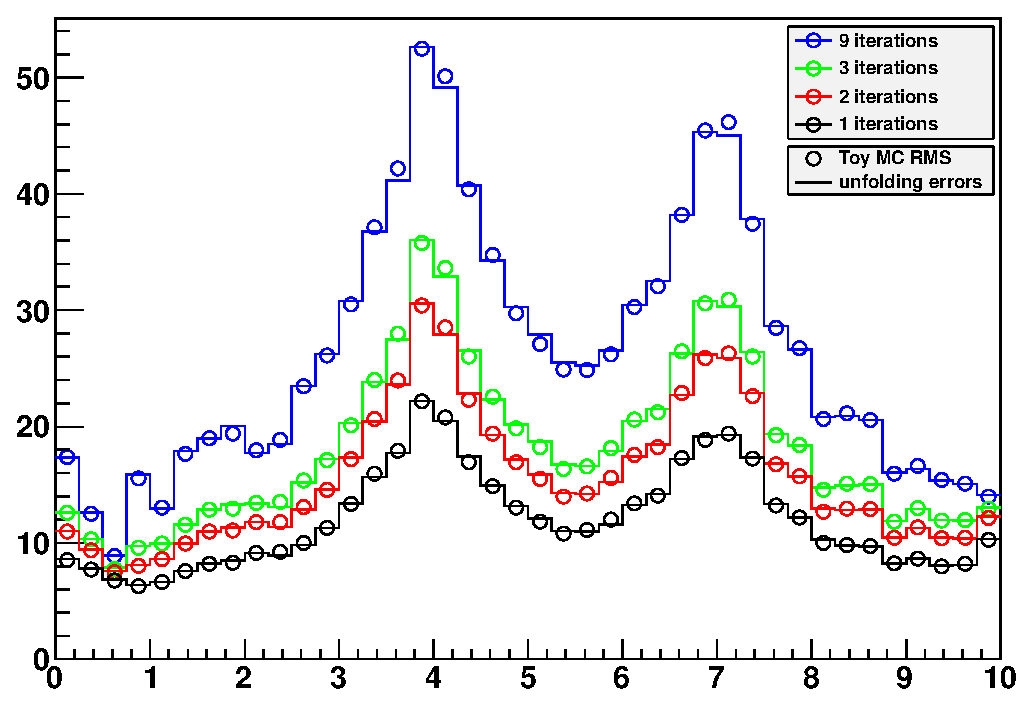
\includegraphics[width=.47\textwidth,clip]{bayes_errors_new.eps}}%
\caption
[Bayesian unfolding errors compared to toy MC]%
{Bayesian unfolding errors compared to toy MC RMS for 1, 2, 3, and 9 iterations.
The left-hand plot shows the errors using D'Agostini's original method,
ignoring any dependence on previous iterations (only the first term of eq.~\ref{eq:dnCidnEj}).
The right-hand plot shows the full error propagation.}%
\label{fig:bayes_errors}%
\end{figure}

D'Agostini takes a multinomial distribution for the bin contents, and hence

\begin{equation}
V(n(\E_i),n(\E_j)) = n(\E_i) \delta_{ij} - \frac{n(\E_i) n(\E_j)}{\hat{N}_{\mathrm{true}}}
\end{equation}

That describes a histogram with the fixed normalisation, ie. fixed total number of measured events.
On the other hand, in counting experiments common in particle physics, each bin is independently Poisson distributed, with

\begin{equation}
V(n(\E_i),n(\E_j)) = n(\E_i) \delta_{ij}
\end{equation}

Other, arbitrary, bin errors (perhaps even correlated) may also be used in equation~\ref{eq:Vij}.

\subsection{Response matrix uncertainties}

The response matrix, $P(\E_j|\C_i)$, is usually estimated by Monte Carlo. If only limited MC statistics
are available, then there will be uncertainties on these terms. Their effect can be determined using

\begin{equation}
\dd{\hat{n}(\C_i)}{P(\E_j|\C_k)} = \frac{n_0(\C_i) n(\E_j)}{f_j \epsilon_i} \left( \delta_{ik} - \frac{n_0(\C_k)}{f_j} \right)
\end{equation}

where here $f_j \equiv \sum_{l=1}^{n_{\C}} P(\E_j|\C_l) n_0(\C_l)$ is the folded prior. The covariance matrix due to these errors is
given by

\begin{equation}
V(\hat{n}(\C_k),\hat{n}(\C_l)) = \sum_{i,r=1}^{n_{\E}} \sum_{j,s=1}^{n_{\C}} \dd{\hat{n}(\C_k)}{P(\E_i|\C_j)} V(P(\E_i|\C_j),P(\E_r|\C_s)) \dd{\hat{n}(\C_l)}{P(\E_r|\C_s)}
\end{equation}

where $V(P(\E_i|\C_j),P(\E_r|\C_s))$ can be taken as multinomial, Poisson, or other distribution.

\begin{thebibliography}{99}

\bibitem{D'Agostini:1994zf}
  G.~D'Agostini,
  ``A Multidimensional unfolding method based on Bayes' theorem,''
  Nucl.\ Instrum.\ Meth.\  A {\bf 362} (1995) 487.
  %%CITATION = NUIMA,A362,487;%%

\bibitem{Multhei:1986ps}
  H.~N.~M\"ulthei and B.~Schorr,
  ``On an Iterative Method for the Unfolding of Spectra,''
  Nucl.\ Instrum.\ Meth.\  A {\bf 257} (1987) 371.
  %%CITATION = NUIMA,A257,371;%%

\end{thebibliography}
\end{document}
